This section describes the deliberation process of the agent based in the practical reasoning theory called BDI (Belief-Desires-Intention) model. This model approach to a reasoning of the agent with limited resources and capabilities, opening the process to the idea of uncertainly which in cases with highly dynamic conditions it have demonstrated to be successful. Understand the BDI model imply understand how its three key features works\cite{Wooldridge2009}.

The beliefs represent knowledge or fact about its environment. In this case, the knowledge was encapsulate by the belief manager, described in previous section. This knowledge can vary on time and in wide range of manners.

The desires are goals that the agent wants to achieve. In a practical point of view the desires represent the ideal state of the world for an agent.

The intentions represent the commitment with the agents some of its desires, it means that the agent not only pursuit the accomplishment of its desires but also plan how to act in concordance to them. Depend on how strong the commitment is, the intention lead the agent to take action.

The BDI model fits perfectly in this work, because the agent architecture aim to generate behavior strongly similar to human behavior. After all, the theater field was developed and practiced only by human beings. Another great feature its the ambiguity in the mental process which the BDI model try to represent. This kind of ambiguity allow to handle uncertainty not only in the action level of an agent, but also in the cognitive level.

\subsection{Goals life-cycle}

The deliberation process is summarized in a simultaneous evaluation of agent's goals, in which the goals acquire different states (see Figure \ref{fig:GoalManager}).

\begin{figure}
	\centering
	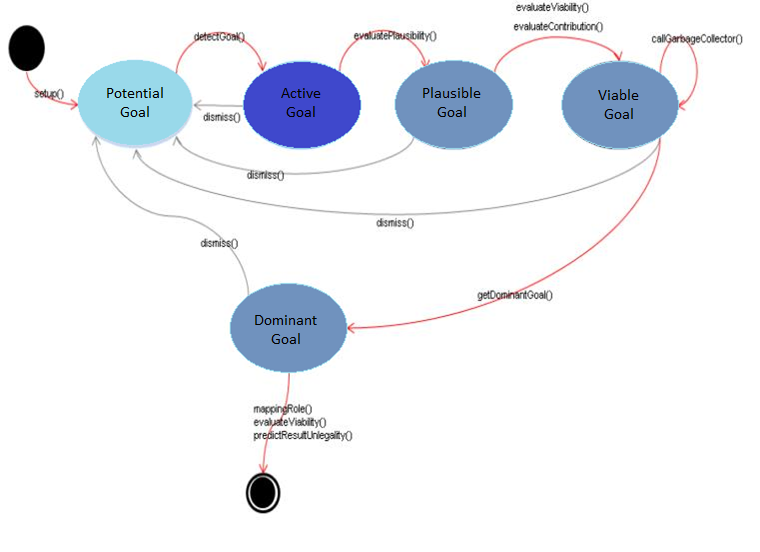
\includegraphics[width=0.5\textwidth]{Images/GoalManagement.png} 
	\caption{GoalManagement. This figure show the goal states in his life-cycle.}
	\label{fig:GoalManager}
\end{figure}

The goals the agent knows are those  delegated by the script and those that are attached to the robotic behaviour, like recharge batteries or preserve its own integrity. These goals receive the name of potential goals. 

When a potential goal satisfies its preconditions the goal becomes an active goal. At this point, the agent check if exists the abilities and resources needed to complete the goal. If not, the goal remains as a potential goal. If there is enough tools and resources the goal becomes a viable goal.

Finally, to the decide what of the viable goals becomes an intention, they compete in two aspects. First, the goals compete by priority, the agent with maximum priority wins. If there is more than one in the maximum priority the goals compete with their contribution values and probability of success (which is an estimated).

\subsection{Resources and Abilities}
Resources are this beliefs that must be true to perform the action. Whilst abilities are those things that the robot can do. Notice that, this beliefs are different from the precondition described in each goal, because this beliefs depends on the platform. 

For example, for the context of a play an actor need to grab an object, but is probable that the robot doesn't have an actuator for accomplish the task. Then the agent doesn't have the ability.

It works in the same way for the resources. For example, for a goal given by the script the unique precondition for the agent to move is that this start at a given position, but probably the agent cannot move because its a differential robot and there is no path for reach the objective. Then this problem its also a lack of resources because in order to reach the point the agent need a given configuration in space to find a path.

Resources and abilities are defined both in the profile action for each simple action. Therefore, the resources and abilities for a specific goal are the union of each simple action in its plan. 

\subsection{Expropriation and Perseverance}

When an goal becomes an intention the agent deal with indecision problems in real-time. The agent handle when an intention is expropriated by another or when it is maintain.

Expropriation occurs naturally in BDI deliberative process. This happens because the current intention still compete as a potential goal. Then, if some other goal becomes an intention automatically take the place of the current intention. On contrast, if the "winner" goal is the current intention, it maintains as an intention.

However to guarantee some commitment of the agent with his current intention the agent gives a boost in goal's contribution value. In this way, the agent show preference for his current intention when have to decide between several goals. However, despite of the boost, clearly the expropriation is still possible, when the contribution level  is significantly less in compare to another goal or the 


\subsection{Plan of actions}
When an goal becomes an intention the agent follows its plan of action. The plan of action is given by the script and incorporated in a delegated goal. This plan of action its represented as a directed graph (See figure).

\begin{figure}
	\centering
	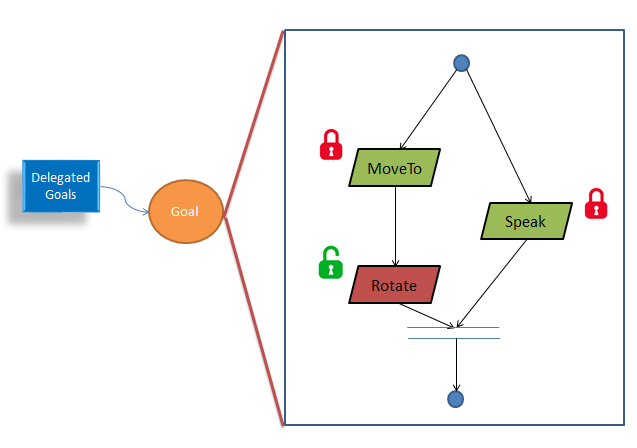
\includegraphics[width=0.5\textwidth]{Images/PlanOfAction.png} 
	\caption{Plan of action. This figure show the simple actions that compose a goal.}
	\label{fig:GoalManager}
\end{figure}

For this purpose the action decision system has a component called action controller. It keeps track of which simple action are executed in a given time.  Then, this plan can be viewed as a state machine in which the controller can pause, cancel or resume a given action. There is a special synchronized barrier (represent by parallel lines) that allows a wait for concurrent paths.

The action controller also handle the resources and abilities access. It means, the action controller acquire and lock the resources and abilities. This allow, an intelligent usage of those and could be managed internally (through its abilities) and externally (through its resources). For resources, the agent sent a global message indicating that this resource is lock.

\subsection{Cooperation Manager}

The cooperation manager is on charge of communication with other robo-actor agents. For this purpose is proposed a specialized channel of communication when the messages are FIPA compliant. Two steps are considered in the process of cooperation, which is included directly influence the BDI model. 

Firstly, a simple step, only through implicit synchronization guided by the script, in which participants are clearly described when a cooperative action is needed.

This first step allow to both agents perceive a specific desire as cooperative, and be ready for negotiation. As it is guided for the script the script has an explicit definition of a cooperative action, with this information the belief system can create the delegated goals marking those who needs cooperation.

The second stage is much more complex and requires a communication protocol that ends with the commitment of parts involved in the cooperation. 

\subsubsection{Protocol for robo-actors}

When an agent set a cooperative delegated goal as a desire immediately search for the ideal partners for achieve it. Then the first message is send  as a petition to the group of ideal partners. At this point every partner cannot reply to the message for lack of interest in the cooperative action or ignorance about the action. at the other hand in the positive case, the agent reply affirmative to the source of petition.

The agent source of the petition acquires the responsibility of determine when the cooperative desire is possible or impossible based on the numbers of agents that have been response willing to cooperate. When the desire becomes possible the agent send a synchronization signal that also works as a commitment message, putting the cooperative desire as an intention

This both steps described above, allows effective coordination within the BDI model. 